\documentclass[10pt]{article}

\def\Type{LessonDJ}
\def\TypeNum{Workshop Week 1} %Lesson #
\def\TypeTitle{Slopes \& Rates of Change } %Lesson Title
\def\Semester{Fall 2021} %Not Used 
\def\Course{MATH 1190 \& 1210}%Course number and name
\def\Targets{ \target{F1} }

\usepackage{preambleDJ} 

%%%%%%%%%%%% BEGIN DOCUMENT %%%%%%%%%%%%%%%
%%%%%%%%%%%% BEGIN DOCUMENT %%%%%%%%%%%%%%%
%%%%%%%%%%%% BEGIN DOCUMENT %%%%%%%%%%%%%%%
%%%%%%%%%%%% BEGIN DOCUMENT %%%%%%%%%%%%%%%
%%%%%%%%%%%% BEGIN DOCUMENT %%%%%%%%%%%%%%%

\begin{document}
\pagestyle{otherpages}
\thispagestyle{firstpage}

\vs{.5}
\section{Exercise A Extra Practice}

\enumA{

\item  Consider the typical Black Friday sale for televisions and suppose that we wished to model the relationship between sale-hungry \textbf{buyers}, $B$ and the availability of cheaply made \textbf{televisions}, $T$. Assume that these things are related and suppose that we have collected two data points $(B_1, T_1) = (10, 1000)$ and $(B_2, T_2) = (100, 100).$
\enumRo{
        \item What is the net change in available televisions from when the buyer population changed from $10$ to $100$ buyers?
        \item What is the average rate of change of the number of available televisions with respect to the number of buyers?
        \item Assuming the buyer-television model is linear, what is the slope of the graph describing the relationship between number of buyers and number of available televisions?
        \item Assuming the buyer-television model is linear, find a function that describes the relationship between between number of buyers and number of available televisions.
}
\item  The equation $\ds N = \frac{10}{9}T + 5$ describes the relationship between the temperature $T$ (in Celsius) and the number of ice cream cones purchased from a supermarket in Charlottesville $N$ (in cones).
	\enumRo{
        \item What is the slope of the graph that describes the relationship between temperature $T$ and number of ice cream comes sold $N?$
        \item What is the (average) rate of change of the number of ice cream comes sold with respect to the change in degrees Celsius?
        \item  What is the net change (rounded down) in the number of ice cream cones sold when the temperature increases by one degree Celsius?
	}

}

\newpage
\section{Exercise A Extra Extra Practice}

\enumA{

\item Suppose that we wished to model the relationship between number of Gophers (the animal, not the sports team), $G$ and the number of holes dug in a garden $H$. Assume that these things are related and suppose that we have collected two data points $(G_1, H_1) = (10, 10)$ and $(G_2, H_2) = (100, 1000).$
   \enumRo{
        \item What is the net change in the number of holes dug from when the gopher population changed from $10$ to $100$?
        \item What is the average rate of change of the number of holes with respect to the number of gophers?
        \item Assuming the gopher-hole model is linear, what is the slope of the graph describing the relationship?
    }
\item At Willie Wonka's Chocolate Factor, the backup holding vat is used to collect overflow from the chocolate river.  The equation $\ds L = \frac{100}{3}T + 1000$ describes the relationship between the the amount of liquid chocolate in liters,  $L$, with respect to  with respect to time,  $T$, in minutes.  
    \enumRo{
        \item  What is the slope of the graph that describes the relationship between $L$ and $T?$
        \item What is the (average) rate of change of the number of the volume of chocolate with respect to time?
        \item  What is the net change (rounded up) in the number of liters in the vat after exactly one additional minute of pumping?
    }

}

\newpage
\section{Exercise B Extra Practice}



The graph below depicts the relationship between temperature in degrees Celsius and temperature in degrees Fahrenheit, with two points plotted to indicate temperatures at which water freezes and at which water boils.

 
\begin{center}
        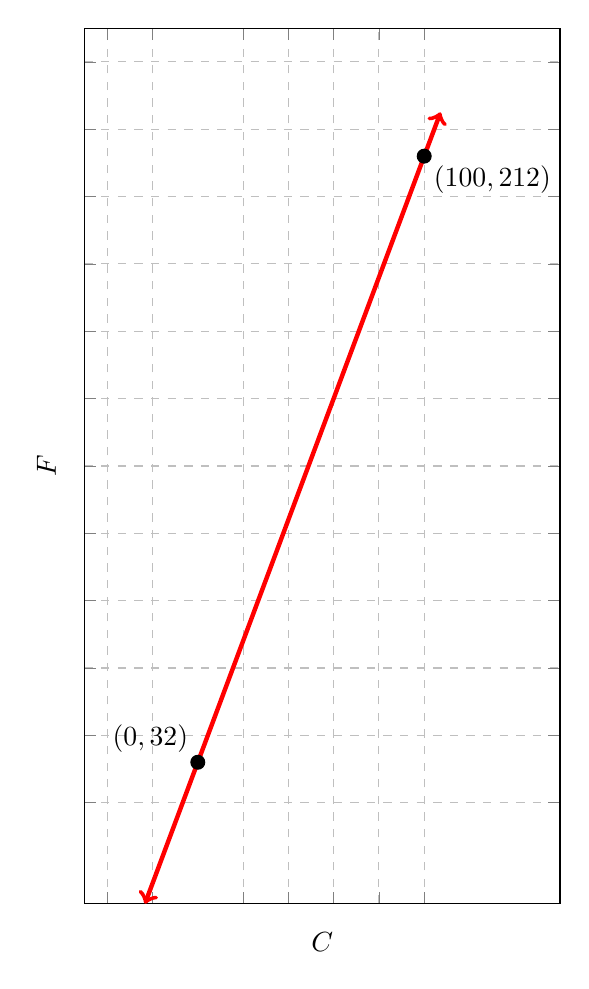
\begin{tikzpicture}
            \begin{axis}[
                %    axis y line = left,
                %    axis x line = bottom,
                    xlabel={$C$},
                    xtick       = {-40,-20,20,40,60,80,100},
                    xticklabels = {},
                    ylabel={$F$},
                    ytick       = {-40,-20,20,40,60,80,100,120,140,160,180,200,220,240},
                    yticklabels = {-40},
                    samples     = 160,
                    %domain      = -1:5,
                    %restrict y to domain=-1:5,
                    ymin = -10, ymax = 250,
                    xmin = -50, xmax = 160,
                    grid=both, grid style=dashed,
                    width=3in, height=5in
                  ]
                  \draw[ultra thick,red,<->] (-23.33333,-10) -- (107.22222222,225);
                  %\filldraw (-40,-40) circle (2.5pt);
                  \filldraw (0,32) circle (2.5pt) node[anchor=south east]{$(0,32)$};
                  \filldraw (100,212) circle (2.5pt) node[anchor=north west]{$(100,212)$};
            \end{axis}
        \end{tikzpicture}
\end{center}

    \enumA{
    
    \item What is the {\bf net change} of the temperature in degrees Fahrenheit as the temperature in degrees Celsius changes from water's freezing point to water's boiling point?
    
    \item What is the {\bf average rate of change} of the temperature in degrees Fahrenheit as the temperature in degrees Celsius changes from water's freezing point to water's boiling point? What are the {\bf units} of measurement of this average rate of change?
    
    \item What is the {\bf slope} of the graph depicted above? What is the {\bf equation} of the graph depicted above?
    
    \item Write a sentence describing what the slope of the graph represents in this context.\\ 
    ({\bf Note:} ``in this context" means your answer must clearly relate to the scenario described in the problem - a graph relating temperature $C$ in degrees Celsius to temperature $F$ in degrees Fahrenheit. Answers like ``rise over run" are not in-context.)

    \item ({\bf Challenge!}) At both the freezing point and boiling point of water, the temperatures in degrees Fahrenheit are numerically greater than the corresponding temperatures in degrees Celsius. Are there any examples of temperatures in degrees Fahrenheit that are numerically {\bf less than} the corresponding temperatures in degrees Celsius? Is there an example of a temperature in degrees Fahrenheit that are numerically {\bf equal} to the corresponding temperature in degrees Celsius? Explain.
    
    }




\newpage
\section{Exercise B Extra Extra Practice}



The graph below depicts the relationship between ounces and pounds with two points plotted.

\begin{center}
        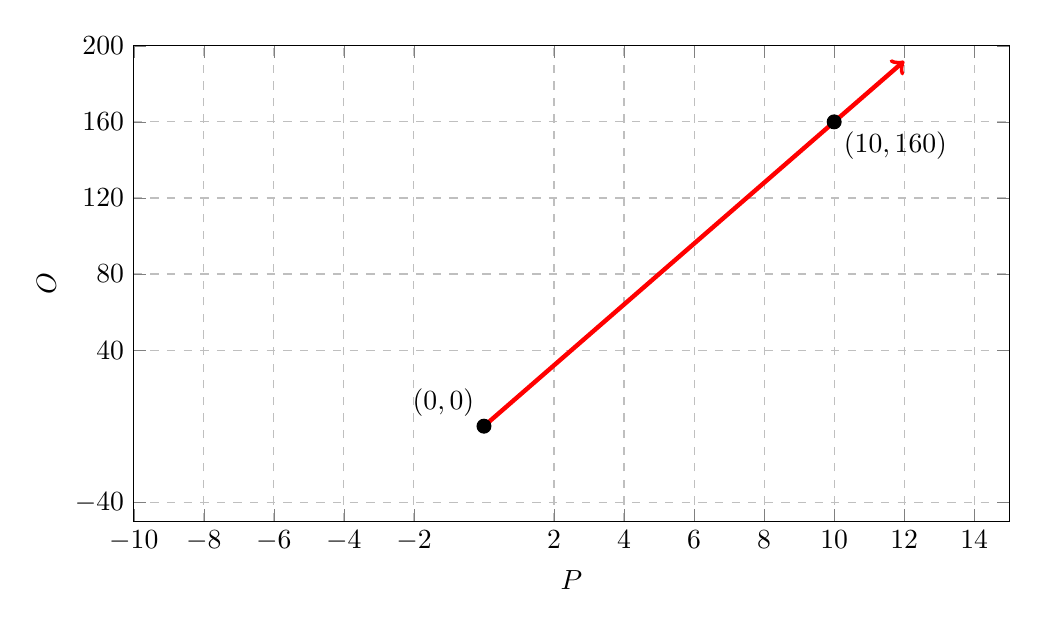
\begin{tikzpicture}
            \begin{axis}[
                %    axis y line = left,
                %    axis x line = bottom,
                    xlabel={$P$},
                    xtick       = {-10,-8,-6,-4,-2,2,4,6,8,10,12,14},
                    %xticklabels = {-40},
                    ylabel={$O$},
                    ytick       = {-40,40,80, 120, 160 ,200},
                    %yticklabels = {},
                    samples     = 160,
                    %domain      = -1:5,
                    %restrict y to domain=-1:5,
                    xmin = -10, xmax = 15,
                    ymin = -50, ymax = 200,
                    grid=both, grid style=dashed,
                    width=5in, height=3in
                  ]
                  \draw[ultra thick,red,->] (0,0) -- (12,192);
                  %\filldraw (-40,-40) circle (2.5pt);
                  \filldraw (0,0) circle (2.5pt) node[anchor=south east]{$(0,0)$};
                  \filldraw (10,160) circle (2.5pt) node[anchor=north west]{$(10,160)$};
            \end{axis}
        \end{tikzpicture}
\end{center}

    \enumA{
    
    \item What is the {\bf net change} of the in ounces with respect to pounds between the marked points?
    
    \item What is the {\bf average rate of change}? What are the {\bf units} of measurement of this average rate of change? 
    
    \item What is the {\bf slope} of the graph depicted above? What is the {\bf equation} of the function that created the graph depicted above?
    
    \item Write a sentence describing what the slope of the graph represents in this context.\\ 
    ({\bf Note:} ``in this context" means your answer must clearly relate to the scenario described in the problem.
    
    }
    \newpage
    \section{Exercise C Extra Practice}
    \mpageT{.6}{.4}{
    The function $\ds y=8-x^3$ has a tangent line located at $(2,0)$ as shown to the right. In this problem we're going to estimate the slope of this tangent line, i.e the  {\em instantaneous rate of change} (IROC) at $x=2$ in two different ways.
    }{
    \begin{flushright}
    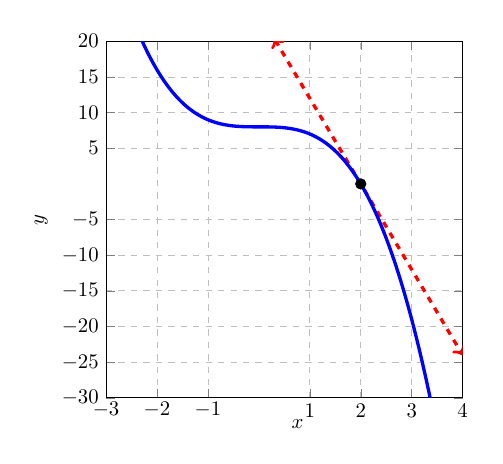
\begin{tikzpicture}[scale=0.75]
	    \begin{axis}[
	        %    axis y line = left,
	        %    axis x line = bottom,
	            xlabel={$x$},
	            xtick       = {-3,-2,-1,1,2,3,4,5},
	            %xticklabels = {},
	             xticklabel  style={yshift=-3ex, anchor=south},
	           %extra x ticks={ 2},
	            %extra x tick labels={$a=2$},
	            extra tick style={grid=none},
	            ylabel={$y$},
	                        xlabel style={anchor=west},
            ylabel style={anchor=south},
	            %ylabel style={anchor=south}.
	            ytick       = {-30,-25,-20,-15,-10,-5,5,10,15,20},
	            %yticklabels = {},
	            samples     = 160,
	            %domain      = -1:5,
	            %restrict y to domain=-1:5,
	            xmin = -3, xmax = 4,
	            ymin = -30, ymax = 20,
	            grid=both, grid style=dashed,
	            width=3in, height=3in
	            ]
	            % curve
	            %\addplot[blue, ultra thick, mark=none, smooth, <->] coordinates{ (0,0) (1,2) (2,3) (3,3) (4,2) (5,.5) };
	            %\draw[ultra thick, red, dashed, <->] (-0.5,0.25) -- (4.75,5.5);
	             \addplot[red, ultra thick, mark=none, dashed, domain=0.3:4, <->] {-12*x+24};
            \addplot[blue, ultra thick, mark=none, smooth, domain=-3:4, ->] {8-x^3};
            \filldraw (2,0) circle (2.5pt);
	    \end{axis}
	\end{tikzpicture}
	\end{flushright}
}
\enumA{
\item Find the average rate of change of $y$ as $x$ changes from $0$ to $2$.\\
\mpageT{.4}{.6}{
    \begin{flushleft}
    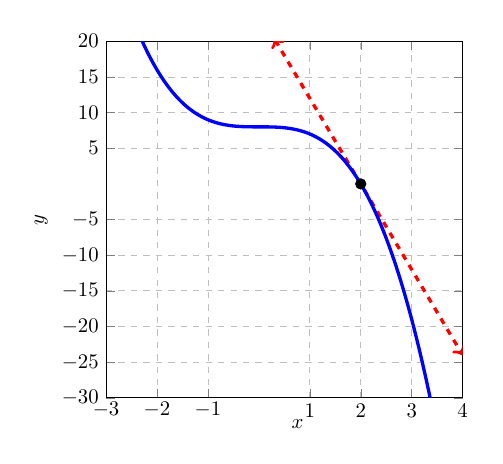
\begin{tikzpicture}[scale=0.75]
	    \begin{axis}[
	        %    axis y line = left,
	        %    axis x line = bottom,
	            xlabel={$x$},
	            xtick       = {-3,-2,-1,1,2,3,4,5},
	            %xticklabels = {},
	             xticklabel  style={yshift=-3ex, anchor=south},
	           %extra x ticks={ 2},
	            %extra x tick labels={$a=2$},
	            extra tick style={grid=none},
	            ylabel={$y$},
	                        xlabel style={anchor=west},
            ylabel style={anchor=south},
	            %ylabel style={anchor=south}.
	            ytick       = {-30,-25,-20,-15,-10,-5,5,10,15,20},
	            %yticklabels = {},
	            samples     = 160,
	            %domain      = -1:5,
	            %restrict y to domain=-1:5,
	            xmin = -3, xmax = 4,
	            ymin = -30, ymax = 20,
	            grid=both, grid style=dashed,
	            width=3in, height=3in
	            ]
	            % curve
	            %\addplot[blue, ultra thick, mark=none, smooth, <->] coordinates{ (0,0) (1,2) (2,3) (3,3) (4,2) (5,.5) };
	            %\draw[ultra thick, red, dashed, <->] (-0.5,0.25) -- (4.75,5.5);
	             \addplot[red, ultra thick, mark=none, dashed, domain=0.3:4, <->] {-12*x+24};
            \addplot[blue, ultra thick, mark=none, smooth, domain=-3:4, ->] {8-x^3};
            \filldraw (2,0) circle (2.5pt);
	    \end{axis}
	\end{tikzpicture}
	\end{flushleft}
}{
\enumRo{
\item Sketch the secant line that has the slope equal to this average rate of change
\item Use the equation $\ds y=8-x^3$ to find the average rate of change as $x$ changes from $0$ to $2$.
}
}
\item Find the average rate of change of $y$ as $x$ changes from $2$ to $3$.\\
\mpageT{.4}{.6}{
    \begin{flushleft}
    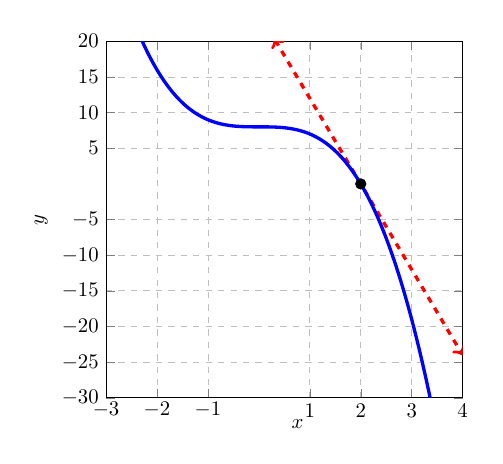
\begin{tikzpicture}[scale=0.75]
	    \begin{axis}[
	        %    axis y line = left,
	        %    axis x line = bottom,
	            xlabel={$x$},
	            xtick       = {-3,-2,-1,1,2,3,4,5},
	            %xticklabels = {},
	             xticklabel  style={yshift=-3ex, anchor=south},
	           %extra x ticks={ 2},
	            %extra x tick labels={$a=2$},
	            extra tick style={grid=none},
	            ylabel={$y$},
	                        xlabel style={anchor=west},
            ylabel style={anchor=south},
	            %ylabel style={anchor=south}.
	            ytick       = {-30,-25,-20,-15,-10,-5,5,10,15,20},
	            %yticklabels = {},
	            samples     = 160,
	            %domain      = -1:5,
	            %restrict y to domain=-1:5,
	            xmin = -3, xmax = 4,
	            ymin = -30, ymax = 20,
	            grid=both, grid style=dashed,
	            width=3in, height=3in
	            ]
	            % curve
	            %\addplot[blue, ultra thick, mark=none, smooth, <->] coordinates{ (0,0) (1,2) (2,3) (3,3) (4,2) (5,.5) };
	            %\draw[ultra thick, red, dashed, <->] (-0.5,0.25) -- (4.75,5.5);
	             \addplot[red, ultra thick, mark=none, dashed, domain=0.3:4, <->] {-12*x+24};
            \addplot[blue, ultra thick, mark=none, smooth, domain=-3:4, ->] {8-x^3};
            \filldraw (2,0) circle (2.5pt);
	    \end{axis}
	\end{tikzpicture}
	\end{flushleft}
}{
\enumRo{
\item Sketch the secant line that has the slope equal to this average rate of change
\item Use the equation $\ds y=8-x^3$ to find the average rate of change as $x$ changes from $2$ to $3$.
}
}
\item Which estimate do you think is closer to the actual IROC? Why?
\item Conceptual Question: If you were to find the average rate of change of $y$ as $x$ changes from $1.5$ to $2$, would you expect this to be closer to the actual IROC than our previous two estimates? Why or why not?  {\bf Note: \em there's no need to compute the average rate of change to answer this question.}
}
    \end{document}